\documentclass{beamer}

\usepackage[utf8]{inputenc}

\AtBeginSection[]
{
  \begin{frame}[noframenumbering,plain]
    \frametitle{Outline for ``\currentsection''}
    \tableofcontents[ 
    currentsubsection, 
    hideothersubsections, 
    sectionstyle=show/shaded
    ] 
  \end{frame}
}

% Allows for refering to the current section name
\newcommand{\currentsection}{}
\newcommand{\mysection}[1]{\renewcommand{\currentsection}{#1}\section{#1}}

\beamertemplateballitem
\usetheme{Antibes}
	\usecolortheme[RGB={120,0,0}]{structure}
	\setbeamertemplate{blocks}[rounded][shadow=true]
%\setbeamertemplate{footline}{\insertframenumber/\inserttotalframenumber}
	\setbeamerfont{page number in head/foot}{size=\large}
	\setbeamertemplate{footline}[frame number]
	\setbeamercovered{transparent=5}
	\setbeamertemplate{navigation symbols}{}
	% To number the references.
	\setbeamertemplate{bibliography item}{\insertbiblabel}

% used to avoid counting references as extra slides
\newcommand{\backupbegin}{
   \newcounter{framenumberappendix}
   \setcounter{framenumberappendix}{\value{framenumber}}
}
\newcommand{\backupend}{
   \addtocounter{framenumberappendix}{-\value{framenumber}}
   \addtocounter{framenumber}{\value{framenumberappendix}} 
}

\usepackage{algorithm}
\usepackage[noend]{algpseudocode}

\usepackage{tikz}
% Define transparent elements
\newcommand{\semitransp}[2][35]{\color{fg!#1}#2\color{fg!100}}
\newcommand{\drawhvector}[5]{
	\edef \origin {#1}
	\edef \xmax {#2}
	\edef \rs {(#3,#4)}
	\edef \scale {#5}
	\foreach \x in {0,...,\xmax}{
		\draw [shift={\origin}] (\x,0) rectangle +\rs;
		\node [scale=\scale, shift={\origin}, font=\LARGE] at (\x + 0.5, 0.5) {\(\x\)};
	}
}
\newcommand{\drawhvectornotext}[5]{
	\edef \origin {#1}
	\edef \xmax {#2}
	\edef \rs {(#3,#4)}
	\edef \scale {#5}
	\foreach \x in {0,...,\xmax}{
		\draw [shift={\origin}] (\x,0) rectangle +\rs;
		%\node [scale=\scale, shift={\origin}, font=\LARGE] at (\x + 0.5, 0.5) {\(\x\)};
	}
}
\newcommand{\drawhvectorfill}[6]{
	\edef \origin {#1}
	\edef \xmax {#2}
	\edef \rs {(#3,#4)}
	\edef \scale {#5}
	\edef \filling {#6}
	\foreach \x in {0,...,\xmax}{
		\draw [shift={\origin},fill=\filling] (\x,0) rectangle +\rs;
		%\node [scale=\scale, shift={\origin}, font=\LARGE] at (\x + 0.5, 0.5) {\(\x\)};
	}
}
\newcommand{\drawaxis}[2]{
	\edef \xmax {#1}
	\edef \ymax {#2}
	\draw [<->, thick] (\xmax,0) -- (0,0) -- (0,\ymax);
	\node [below, font=\small] at (\xmax/2, 0) {weight};
	\node [rotate=90, above, font=\small] at (0,\xmax/2) {profit};
}
\newcommand{\dominate}[3]{
	\edef \xx {#1}
	\edef \yy {#2}
	\edef \xmax {#3}
	\draw [dashed] (\xx, 0) -- (\xx,\yy) -- (\xmax,\yy);
}

% Change the spacing in a 'table of contents'/outline
\usepackage{etoolbox} % allows patching macros
\makeatletter
\patchcmd{\beamer@sectionintoc}{\vskip1.5em}{\vskip0.5em}{}{}
\makeatother

\begin{document}

\title{Unbounded Knapsack Problem: a critical review}
\author{Henrique Becker}
%\logo{
\includegraphics[scale=0.2]{inf}}
\date{Friday, December 16, 2016}

{
	\setbeamertemplate{footline}{} 
	\begin{frame}[noframenumbering]
	\titlepage
	\end{frame}
}

% LAST THING TODO: create a list of topics and copy it between each section
{
	\setbeamertemplate{footline}{} 
	\begin{frame}[noframenumbering]
	\frametitle{Outline}
	\tableofcontents[hideallsubsections] 
	\end{frame}
}

\mysection{Introduction}
\frame{\frametitle{What is UKP?}
\begin{itemize}
%\setlength\itemsep{1.5em}
%\item UKP is an acronym for Unbounded Knapsack Problem.
\item Very similar to BKP or 0-1 KP.
\begin{itemize}
\item But with an ``unbounded'' quantity of each item available.
\end{itemize}
\end{itemize}
\large
\begin{align}
  maximize &\sum_{i=1}^n p_i x_i\label{eq:objfun}\\
subject~to &\sum_{i=1}^n w_i x_i \leq c\label{eq:capcons}\\
            &x_i \in \mathbb{N}_0\label{eq:x_integer}
\end{align}
\normalsize
\begin{itemize}
\vspace{-7mm}
\item Subproblem of the column generation technique applied to the Cutting Stock Problem or the Bin Packing Problem.
\end{itemize}
}

\mysection{Exploitable Properties of the UKP}
\subsection{Dominance Relations}
\frame{\frametitle{A simple (and reusable) example}

\center
\edef \scale {0.25}
\edef \myrad {0.25}
\begin{tikzpicture}[scale=\scale]

\drawaxis{25}{25}

\draw [fill] (3, 2) circle [radius=\myrad];
\draw [fill] (5, 5) circle [radius=\myrad];
\draw [fill] (7, 2) circle [radius=\myrad];
\draw [fill] (11, 4) circle [radius=\myrad];
\draw [fill] (12, 9) circle [radius=\myrad];
\draw [fill] (14, 11) circle [radius=\myrad];
\draw [fill] (16, 13) circle [radius=\myrad];
\draw [fill] (17, 21) circle [radius=\myrad];

\end{tikzpicture}
}

\frame{\frametitle{Simple Dominance}

\center
\edef \scale {0.25}
\edef \myrad {0.25}
\begin{tikzpicture}[scale=\scale]

\drawaxis{25}{25}

\draw [fill] (3, 2) circle [radius=\myrad];
\draw [fill] (5, 5) circle [radius=\myrad];
\draw [fill=red] (7, 2) circle [radius=\myrad];
\draw [fill=red] (11, 4) circle [radius=\myrad];
\draw [fill] (12, 9) circle [radius=\myrad];
\draw [fill] (14, 11) circle [radius=\myrad];
\draw [fill] (16, 13) circle [radius=\myrad];
\draw [fill] (17, 21) circle [radius=\myrad];

\draw [dashed] (5, 0) -- (5, 5) -- (25, 5);

\end{tikzpicture}
}

\frame{\frametitle{Multiple dominance}

\center
\edef \scale {0.25}
\edef \myrad {0.25}
\begin{tikzpicture}[scale=\scale]

\drawaxis{25}{25}

\draw [fill] (3, 2) circle [radius=\myrad];

\draw [blue] (0, 0) -- (15,15);
\draw [fill] (5, 5) circle [radius=\myrad];
\node [above left, font=\tiny] at (5, 5) {(5, 5)};

\draw [dashed] (10, 0) -- (10, 10) -- (25, 10);
\draw [blue,fill=white] (10, 10) circle [radius=\myrad];
\node [above left, font=\tiny] at (10, 10) {(10, 10)};

\draw [dashed] (15, 0) -- (15, 15) -- (25, 15);
\draw [blue,fill=white] (15, 15) circle [radius=\myrad];
\node [above left, font=\tiny] at (15, 15) {(15, 15)};

\draw [fill=red] (7, 2) circle [radius=\myrad];
\draw [fill=red] (11, 4) circle [radius=\myrad];
\draw [fill=red] (12, 9) circle [radius=\myrad];
\draw [fill] (14, 11) circle [radius=\myrad];
\draw [fill=red] (16, 13) circle [radius=\myrad];
\draw [fill] (17, 23) circle [radius=\myrad];

\end{tikzpicture}
}


\frame{\frametitle{Collective dominance}

\center
\edef \scale {0.25}
\edef \myrad {0.25}
\begin{tikzpicture}[scale=\scale]

\drawaxis{25}{25}

\draw [fill] (3, 2) circle [radius=\myrad];
\node [below, font=\tiny] at (3, 2) {(3, 2)};

\draw [blue] (0,0) -- (10,10) -- (13,12);
\draw [fill] (5, 5) circle [radius=\myrad];
\node [above left, font=\tiny] at (5, 5) {(5, 5)};

\draw [blue,fill=white] (10, 10) circle [radius=\myrad];
\node [above left, font=\tiny] at (10, 10) {(10, 10)};

\draw [dashed] (13, 0) -- (13, 12) -- (25, 12);
\draw [blue,fill=white] (13, 12) circle [radius=\myrad];
\node [above left, font=\tiny] at (13, 12) {(13, 12)};

\draw [fill=red] (7, 2) circle [radius=\myrad];
\draw [fill=red] (11, 4) circle [radius=\myrad];
\draw [fill=red] (12, 9) circle [radius=\myrad];
\draw [fill=red] (14, 11) circle [radius=\myrad];
\draw [fill=red] (16, 13) circle [radius=\myrad];
\draw [fill] (17, 21) circle [radius=\myrad];

\end{tikzpicture}
}

\frame{\frametitle{Threshold dominance}

\center
\edef \scale {0.25}
\edef \myrad {0.25}
\begin{tikzpicture}[scale=\scale]

\drawaxis{25}{25}

\draw [dashed] (5, 0) -- (5, 5) -- (25, 5);
\draw [blue] (0,0) -- (6,4);
\node [below, font=\tiny] at (3, 2) {(3, 2)};
\draw [fill] (3, 2) circle [radius=\myrad];
\node [right, font=\tiny] at (6, 4) {(6, 4)};
\draw [blue,fill=red] (6, 4) circle [radius=\myrad];

\draw [blue] (0, 0) -- (20,20);
\draw [fill] (5, 5) circle [radius=\myrad];
\node [above left, font=\tiny] at (5, 5) {(5, 5)};

\draw [blue,fill=white] (10, 10) circle [radius=\myrad];
\node [above left, font=\tiny] at (10, 10) {(10, 10)};

\draw [blue,fill=white] (15, 15) circle [radius=\myrad];
\node [above left, font=\tiny] at (15, 15) {(15, 15)};

\draw [blue,fill=red] (20, 20) circle [radius=\myrad];
\node [above, font=\tiny] at (20, 20) {(20, 20)};

\draw [fill=red] (7, 2) circle [radius=\myrad];
\draw [fill=red] (11, 4) circle [radius=\myrad];
\draw [fill=red] (12, 9) circle [radius=\myrad];
\draw [fill=red] (14, 11) circle [radius=\myrad];
\draw [fill=red] (16, 13) circle [radius=\myrad];

\node [above, font=\tiny] at (17, 23) {(17, 23)};
\draw [fill] (17, 23) circle [radius=\myrad];
\draw [dashed] (17, 0) -- (17, 23) -- (25, 23);

\end{tikzpicture}
}

\frame{\frametitle{Solution dominance}

\center
\edef \scale {0.25}
\edef \myrad {0.25}
\begin{tikzpicture}[scale=\scale]

\drawaxis{25}{25}

\node [below, font=\tiny] at (3, 2) {(3, 2)};
\draw [fill] (3, 2) circle [radius=\myrad];

\draw [blue] (0, 0) -- (15,15) -- (18,17);
\draw [fill] (5, 5) circle [radius=\myrad];
\node [above left, font=\tiny] at (5, 5) {(5, 5)};

\draw [blue,fill=white] (10, 10) circle [radius=\myrad];
\node [above left, font=\tiny] at (10, 10) {(10, 10)};

\draw [blue,fill=white] (15, 15) circle [radius=\myrad];
\node [above left, font=\tiny] at (15, 15) {(15, 15)};

\draw [blue,fill=red] (18, 17) circle [radius=\myrad];
\node [right, font=\tiny] at (18,17) {(18, 17)};

\draw [fill=red] (7, 2) circle [radius=\myrad];
\draw [fill=red] (11, 4) circle [radius=\myrad];
\draw [fill=red] (12, 9) circle [radius=\myrad];
\draw [fill=red] (14, 11) circle [radius=\myrad];
\draw [fill=red] (16, 13) circle [radius=\myrad];

\draw [blue,fill=red,opacity=0.25] (6, 4) circle [radius=\myrad];
\draw [blue,fill=red,opacity=0.25] (20, 20) circle [radius=\myrad];

\node [above, font=\tiny] at (17, 23) {(17, 23)};
\draw [fill] (17, 23) circle [radius=\myrad];
\draw [dashed] (17, 0) -- (17, 23) -- (25, 23);

\end{tikzpicture}
}

\subsection{Periodicity}
\frame{\frametitle{Periodicity and Threshold Dominance}

\center
\edef \scale {0.25}
\edef \myrad {0.25}
\begin{tikzpicture}[scale=\scale]

\drawaxis{25}{25}

\draw [blue] (0,0) -- (6,4);
\draw [dashed] (5,0) -- (5,5) -- (25,5);
\draw [fill] (3, 2) circle [radius=\myrad];
\draw [blue,fill=red] (6, 4) circle [radius=\myrad];

\draw [blue] (0,0) -- (15,15);
\draw [dashed] (14,0) -- (14,16) -- (25,16);
\draw [fill] (5, 5) circle [radius=\myrad];
\draw [blue,fill=white] (10, 10) circle [radius=\myrad];
\draw [blue,fill=red] (15, 15) circle [radius=\myrad];

\draw [blue] (0,0) -- (21,24);
\draw [dashed] (20,0) -- (20,25) -- (25,25);
\draw [fill] (7, 8) circle [radius=\myrad];
\draw [blue,fill=white] (14, 16) circle [radius=\myrad];
\draw [blue,fill=red] (21, 24) circle [radius=\myrad];

\draw [blue,->] (0,0) -- (20.8,26);
\draw [fill] (20, 25) circle [radius=\myrad];

\end{tikzpicture}
}

\frame{\frametitle{Periodicity and bounds in \(x_i\)}

\center
\edef \scale {0.25}
\edef \myrad {0.25}
\begin{tikzpicture}[scale=\scale]

\drawaxis{25}{25}

\draw [blue,fill=white] (0,0) -- (3,2);
\draw [fill] (3, 2) circle [radius=\myrad];
\node [right, font=\tiny] at (3,2) {\(x_4 \leq 1\)};

\draw [blue] (0,0) -- (10,10);
\draw [fill] (5, 5) circle [radius=\myrad];
\draw [blue,fill=white] (10, 10) circle [radius=\myrad];
\node [right, font=\tiny] at (10,10) {\(x_3 \leq 2\)};

\draw [blue] (0,0) -- (14,16);
\draw [fill] (7, 8) circle [radius=\myrad];
\draw [blue,fill=white] (14, 16) circle [radius=\myrad];
\node [right, font=\tiny] at (14, 16) {\(x_2 \leq 2\)};

\draw [blue,->] (0,0) -- (20.8,26);
\draw [fill] (20, 25) circle [radius=\myrad];
\node [left, font=\tiny] at (20, 25) {\(x_1 \in [0, \infty)\)};

\end{tikzpicture}
}

\frame{\frametitle{Periodicity and an upper bound on \(y^+\)}

\center
\edef \scale {0.15}
\edef \myrad {0.5}
\begin{tikzpicture}[scale=\scale]

\drawaxis{25}{25}
\draw [<->, thick] (40,0) -- (0,0) -- (0,40);

\draw [fill] (5, 5) circle [radius=\myrad];
\draw [fill] (7, 8) circle [radius=\myrad];

\draw [dashed] (27,0) -- (27,40);
\node [right, font=\tiny, align=left] at (27,15) {\(y^+ \leq 2 w_2 + 2 w_3 + w_1\)};

\draw [blue] (0,0) -- (3,2) -- (13,12) -- (27,28);
\draw [fill] (3, 2) circle [radius=\myrad];
\node [right, font=\tiny] at (3,2) {\(x_4 = 1\)};

\draw [blue,fill=white] (8, 7) circle [radius=\myrad];
\draw [blue,fill=white] (13, 12) circle [radius=\myrad];
\node [right, font=\tiny, align=left] at (13,12) {\(x_3 = 2~\&\) \\ \(x_4 = 1\)};

\draw [blue,fill=white] (20, 20) circle [radius=\myrad];
\draw [blue,fill=white] (27, 28) circle [radius=\myrad];
\node [right, font=\tiny, align=left] at (27,28) {\(x_2 = 2~\&\) \\ \(x_3 = 2~\&\) \\ \(x_4 = 1\)};

\draw [blue,->] (0,0) -- (30,37.5);
\draw [fill] (20, 25) circle [radius=\myrad];

\end{tikzpicture}
}

\mysection{Prior Work}
\begin{frame}[allowframebreaks]{Prior Work}
\begin{description}
\item[1961] A real-world application of the UKP is proposed.\cite{gg-61} % say that's the BPP and CSP
\item[1966] DP algorithms for such application are proposed.\cite{gg-66} % says dynamic programming
\item[1977] A B\&B method is proposed, and then compared with the DP algorithms over small artificial instances, obtaining marginally better results.\cite{mtu1} % says that's MTU1? say that the original benchmark using real world instances was already abandoned
\item[1990] The goal changes to solving larger instances faster. Artificial datasets are used for this. For such datasets, DP methods are clearly dominated by B\&B methods.\cite{mtu2} % we don't know if there's real world instances of the UKP so large as these artificial datasets
\item[1997] The large artificial instances are shown to have only a little amount of relevant/undominated items and are discredited.\cite{zhu_dominated} % we will see more about this in the future
\item[1998] A new DP method is proposed, together with new artificial datasets (without the same flaws of the previous datasets).\cite{ukp_new_results} % the return to the application didn't occur
\item[2000] The new DP method only compares to B\&B and naive DP.\cite{eduk} % the old non-naive DP algorithms were forgotten or excluded because of previous experiments.
\item[2004] A PhD thesis on KP's consider the method to be the state-of-the-art DP for UKP.\cite{book_ukp_2004}
\item[2009] The new DP method is hybridized with B\&B, and the datasets are updated to be `harder'. Such datasets are hard for B\&B, and the hybrid method is only compares with B\&B.\cite{pya} % say "The hybrid method is the new state-of-the-art, as it clearly improves the old algorithm that was considered state-of-the-art."
\item[2016] An old DP method is reinvented and outperforms the hybrid method in the updated datasets.\cite{sea2016}
\end{description}
\end{frame}

\frame{\frametitle{Current Work}
\centering
\begin{description}
\item[(this thesis)] Old algorithms are implemented and tested. The influence of the datasets in the comparisons becomes apparent.
\end{description}
}

\mysection{The Instance Classes}

\frame{\frametitle{The Instance Classes}
\begin{itemize}
\item The majority of the UKP instances in the literature is artificial.
\item The items distribution has a strong effect in the instance hardness.
\item An efficient method for some dataset can be inefficient for another.
  \begin{itemize}
    \item Specially: efficient algorithms for some artificial dataset can be inefficient for real-world datasets and vice-versa.
  \end{itemize}
\end{itemize}
}

\subsection{Discredited and not used}

\frame{\frametitle{Uncorrelated}
\center
\edef \scale {0.60}
\edef \myrad {0.125}
\begin{tikzpicture}[scale=\scale]

\drawaxis{10}{10}

\draw[fill] (0.01, 7.85) circle [radius=\myrad];
\draw[fill] (0.02, 7.7) circle [radius=\myrad];
\draw[fill] (0.04, 8.51) circle [radius=\myrad];
\draw[fill] (0.08, 8.25) circle [radius=\myrad];
\draw[fill] (0.08, 8.22) circle [radius=\myrad];
\draw[fill] (0.38, 4.65) circle [radius=\myrad];
\draw[fill] (0.39, 6.79) circle [radius=\myrad];
\draw[fill] (0.43, 7.3) circle [radius=\myrad];
\draw[fill] (0.83, 7.2) circle [radius=\myrad];
\draw[fill] (0.86, 1.34) circle [radius=\myrad];
\draw[fill] (0.9, 7.94) circle [radius=\myrad];
\draw[fill] (1.18, 3.56) circle [radius=\myrad];
\draw[fill] (1.35, 7.34) circle [radius=\myrad];
\draw[fill] (1.39, 4.11) circle [radius=\myrad];
\draw[fill] (1.41, 4.12) circle [radius=\myrad];
\draw[fill] (1.58, 8.63) circle [radius=\myrad];
\draw[fill] (1.72, 0.3) circle [radius=\myrad];
\draw[fill] (1.9, 1.8) circle [radius=\myrad];
\draw[fill] (1.98, 4.28) circle [radius=\myrad];
\draw[fill] (2.08, 1.14) circle [radius=\myrad];
\draw[fill] (2.09, 1.29) circle [radius=\myrad];
\draw[fill] (2.17, 4.15) circle [radius=\myrad];
\draw[fill] (2.34, 9.18) circle [radius=\myrad];
\draw[fill] (2.41, 1.87) circle [radius=\myrad];
\draw[fill] (2.56, 4.53) circle [radius=\myrad];
\draw[fill] (2.62, 1.36) circle [radius=\myrad];
\draw[fill] (2.72, 4.52) circle [radius=\myrad];
\draw[fill] (2.87, 2.17) circle [radius=\myrad];
\draw[fill] (3.06, 2.88) circle [radius=\myrad];
\draw[fill] (3.34, 7.2) circle [radius=\myrad];
\draw[fill] (3.34, 5.32) circle [radius=\myrad];
\draw[fill] (3.47, 3.25) circle [radius=\myrad];
\draw[fill] (3.6, 3.17) circle [radius=\myrad];
\draw[fill] (3.76, 5.93) circle [radius=\myrad];
\draw[fill] (3.8, 1.49) circle [radius=\myrad];
\draw[fill] (3.89, 6.32) circle [radius=\myrad];
\draw[fill] (3.91, 9.2) circle [radius=\myrad];
\draw[fill] (3.99, 7.79) circle [radius=\myrad];
\draw[fill] (4.32, 7.34) circle [radius=\myrad];
\draw[fill] (4.36, 0.81) circle [radius=\myrad];
\draw[fill] (4.47, 2.34) circle [radius=\myrad];
\draw[fill] (4.58, 6.09) circle [radius=\myrad];
\draw[fill] (4.63, 5.36) circle [radius=\myrad];
\draw[fill] (4.75, 6.13) circle [radius=\myrad];
\draw[fill] (4.8, 4.81) circle [radius=\myrad];
\draw[fill] (5.15, 7.95) circle [radius=\myrad];
\draw[fill] (5.15, 6.81) circle [radius=\myrad];
\draw[fill] (5.15, 3.95) circle [radius=\myrad];
\draw[fill] (5.16, 1.13) circle [radius=\myrad];
\draw[fill] (5.2, 9.63) circle [radius=\myrad];
\draw[fill] (5.61, 8.29) circle [radius=\myrad];
\draw[fill] (5.64, 7.48) circle [radius=\myrad];
\draw[fill] (5.67, 1.97) circle [radius=\myrad];
\draw[fill] (5.82, 9.19) circle [radius=\myrad];
\draw[fill] (6.12, 6.24) circle [radius=\myrad];
\draw[fill] (6.19, 1.5) circle [radius=\myrad];
\draw[fill] (6.2, 7.32) circle [radius=\myrad];
\draw[fill] (6.4, 9.45) circle [radius=\myrad];
\draw[fill] (6.42, 9.43) circle [radius=\myrad];
\draw[fill] (6.46, 2.6) circle [radius=\myrad];
\draw[fill] (6.57, 5.36) circle [radius=\myrad];
\draw[fill] (6.68, 1.95) circle [radius=\myrad];
\draw[fill] (6.76, 9.35) circle [radius=\myrad];
\draw[fill] (6.78, 1.88) circle [radius=\myrad];
\draw[fill] (6.86, 9.38) circle [radius=\myrad];
\draw[fill] (6.94, 1.17) circle [radius=\myrad];
\draw[fill] (7.06, 0.03) circle [radius=\myrad];
\draw[fill] (7.2, 8.37) circle [radius=\myrad];
\draw[fill] (7.2, 1.37) circle [radius=\myrad];
\draw[fill] (7.35, 0.54) circle [radius=\myrad];
\draw[fill] (7.37, 7.4) circle [radius=\myrad];
\draw[fill] (7.38, 9.04) circle [radius=\myrad];
\draw[fill] (7.44, 7.44) circle [radius=\myrad];
\draw[fill] (7.49, 7.76) circle [radius=\myrad];
\draw[fill] (7.6, 6.02) circle [radius=\myrad];
\draw[fill] (7.76, 7.43) circle [radius=\myrad];
\draw[fill] (7.85, 3.95) circle [radius=\myrad];
\draw[fill] (8.12, 6.04) circle [radius=\myrad];
\draw[fill] (8.29, 3.18) circle [radius=\myrad];
\draw[fill] (8.31, 3.89) circle [radius=\myrad];
\draw[fill] (8.33, 5.8) circle [radius=\myrad];
\draw[fill] (8.37, 7.25) circle [radius=\myrad];
\draw[fill] (8.5, 5.36) circle [radius=\myrad];
\draw[fill] (8.88, 1.71) circle [radius=\myrad];
\draw[fill] (9.05, 3.57) circle [radius=\myrad];
\draw[fill] (9.06, 9.63) circle [radius=\myrad];
\draw[fill] (9.07, 7.65) circle [radius=\myrad];
\draw[fill] (9.15, 6.27) circle [radius=\myrad];
\draw[fill] (9.26, 0.73) circle [radius=\myrad];
\draw[fill] (9.34, 1.3) circle [radius=\myrad];
\draw[fill] (9.35, 7.52) circle [radius=\myrad];
\draw[fill] (9.38, 2.18) circle [radius=\myrad];
\draw[fill] (9.41, 5.38) circle [radius=\myrad];
\draw[fill] (9.47, 5.9) circle [radius=\myrad];
\draw[fill] (9.58, 8.18) circle [radius=\myrad];
\draw[fill] (9.71, 2.94) circle [radius=\myrad];
\draw[fill] (9.74, 7.8) circle [radius=\myrad];
\draw[fill] (9.79, 0.02) circle [radius=\myrad];
\draw[fill] (9.83, 5.51) circle [radius=\myrad];
\draw[fill] (9.89, 5.74) circle [radius=\myrad];
\end{tikzpicture}
}

\frame{\frametitle{Uncorrelated}
\center
\edef \scale {0.60}
\edef \myrad {0.125}
\begin{tikzpicture}[scale=\scale]

\drawaxis{10}{10}

\dominate{0.01}{7.85}{10}
\draw[fill] (0.01, 7.85) circle [radius=\myrad];
\dominate{0.02}{7.7}{10};
\draw[fill] (0.02, 7.7) circle [radius=\myrad];
\dominate{0.04}{8.51}{10};
\draw[fill] (0.04, 8.51) circle [radius=\myrad];
\draw[fill=red] (0.08, 8.25) circle [radius=\myrad];
\draw[fill=red] (0.08, 8.22) circle [radius=\myrad];
\draw[fill=red] (0.38, 4.65) circle [radius=\myrad];
\draw[fill=red] (0.39, 6.79) circle [radius=\myrad];
\draw[fill=red] (0.43, 7.3) circle [radius=\myrad];
\draw[fill=red] (0.83, 7.2) circle [radius=\myrad];
\draw[fill=red] (0.86, 1.34) circle [radius=\myrad];
\draw[fill=red] (0.9, 7.94) circle [radius=\myrad];
\draw[fill=red] (1.18, 3.56) circle [radius=\myrad];
\draw[fill=red] (1.35, 7.34) circle [radius=\myrad];
\draw[fill=red] (1.39, 4.11) circle [radius=\myrad];
\draw[fill=red] (1.41, 4.12) circle [radius=\myrad];
\dominate{1.58}{8.63}{10};
\draw[fill] (1.58, 8.63) circle [radius=\myrad];
\draw[fill=red] (1.72, 0.3) circle [radius=\myrad];
\draw[fill=red] (1.9, 1.8) circle [radius=\myrad];
\draw[fill=red] (1.98, 4.28) circle [radius=\myrad];
\draw[fill=red] (2.08, 1.14) circle [radius=\myrad];
\draw[fill=red] (2.09, 1.29) circle [radius=\myrad];
\draw[fill=red] (2.17, 4.15) circle [radius=\myrad];
\dominate{2.34}{9.18}{10};
\draw[fill] (2.34, 9.18) circle [radius=\myrad];
\draw[fill=red] (2.41, 1.87) circle [radius=\myrad];
\draw[fill=red] (2.56, 4.53) circle [radius=\myrad];
\draw[fill=red] (2.62, 1.36) circle [radius=\myrad];
\draw[fill=red] (2.72, 4.52) circle [radius=\myrad];
\draw[fill=red] (2.87, 2.17) circle [radius=\myrad];
\draw[fill=red] (3.06, 2.88) circle [radius=\myrad];
\draw[fill=red] (3.34, 7.2) circle [radius=\myrad];
\draw[fill=red] (3.34, 5.32) circle [radius=\myrad];
\draw[fill=red] (3.47, 3.25) circle [radius=\myrad];
\draw[fill=red] (3.6, 3.17) circle [radius=\myrad];
\draw[fill=red] (3.76, 5.93) circle [radius=\myrad];
\draw[fill=red] (3.8, 1.49) circle [radius=\myrad];
\draw[fill=red] (3.89, 6.32) circle [radius=\myrad];
\dominate{3.91}{9.2}{10};
\draw[fill] (3.91, 9.2) circle [radius=\myrad];
\draw[fill=red] (3.99, 7.79) circle [radius=\myrad];
\draw[fill=red] (4.32, 7.34) circle [radius=\myrad];
\draw[fill=red] (4.36, 0.81) circle [radius=\myrad];
\draw[fill=red] (4.47, 2.34) circle [radius=\myrad];
\draw[fill=red] (4.58, 6.09) circle [radius=\myrad];
\draw[fill=red] (4.63, 5.36) circle [radius=\myrad];
\draw[fill=red] (4.75, 6.13) circle [radius=\myrad];
\draw[fill=red] (4.8, 4.81) circle [radius=\myrad];
\draw[fill=red] (5.15, 7.95) circle [radius=\myrad];
\draw[fill=red] (5.15, 6.81) circle [radius=\myrad];
\draw[fill=red] (5.15, 3.95) circle [radius=\myrad];
\draw[fill=red] (5.16, 1.13) circle [radius=\myrad];
\dominate{5.2}{9.63}{10};
\draw[fill] (5.2, 9.63) circle [radius=\myrad];
\draw[fill=red] (5.61, 8.29) circle [radius=\myrad];
\draw[fill=red] (5.64, 7.48) circle [radius=\myrad];
\draw[fill=red] (5.67, 1.97) circle [radius=\myrad];
\draw[fill=red] (5.82, 9.19) circle [radius=\myrad];
\draw[fill=red] (6.12, 6.24) circle [radius=\myrad];
\draw[fill=red] (6.19, 1.5) circle [radius=\myrad];
\draw[fill=red] (6.2, 7.32) circle [radius=\myrad];
\draw[fill=red] (6.4, 9.45) circle [radius=\myrad];
\draw[fill=red] (6.42, 9.43) circle [radius=\myrad];
\draw[fill=red] (6.46, 2.6) circle [radius=\myrad];
\draw[fill=red] (6.57, 5.36) circle [radius=\myrad];
\draw[fill=red] (6.68, 1.95) circle [radius=\myrad];
\draw[fill=red] (6.76, 9.35) circle [radius=\myrad];
\draw[fill=red] (6.78, 1.88) circle [radius=\myrad];
\draw[fill=red] (6.86, 9.38) circle [radius=\myrad];
\draw[fill=red] (6.94, 1.17) circle [radius=\myrad];
\draw[fill=red] (7.06, 0.03) circle [radius=\myrad];
\draw[fill=red] (7.2, 8.37) circle [radius=\myrad];
\draw[fill=red] (7.2, 1.37) circle [radius=\myrad];
\draw[fill=red] (7.35, 0.54) circle [radius=\myrad];
\draw[fill=red] (7.37, 7.4) circle [radius=\myrad];
\draw[fill=red] (7.38, 9.04) circle [radius=\myrad];
\draw[fill=red] (7.44, 7.44) circle [radius=\myrad];
\draw[fill=red] (7.49, 7.76) circle [radius=\myrad];
\draw[fill=red] (7.6, 6.02) circle [radius=\myrad];
\draw[fill=red] (7.76, 7.43) circle [radius=\myrad];
\draw[fill=red] (7.85, 3.95) circle [radius=\myrad];
\draw[fill=red] (8.12, 6.04) circle [radius=\myrad];
\draw[fill=red] (8.29, 3.18) circle [radius=\myrad];
\draw[fill=red] (8.31, 3.89) circle [radius=\myrad];
\draw[fill=red] (8.33, 5.8) circle [radius=\myrad];
\draw[fill=red] (8.37, 7.25) circle [radius=\myrad];
\draw[fill=red] (8.5, 5.36) circle [radius=\myrad];
\draw[fill=red] (8.88, 1.71) circle [radius=\myrad];
\draw[fill=red] (9.05, 3.57) circle [radius=\myrad];
\draw[fill=red] (9.06, 9.63) circle [radius=\myrad];
\draw[fill=red] (9.07, 7.65) circle [radius=\myrad];
\draw[fill=red] (9.15, 6.27) circle [radius=\myrad];
\draw[fill=red] (9.26, 0.73) circle [radius=\myrad];
\draw[fill=red] (9.34, 1.3) circle [radius=\myrad];
\draw[fill=red] (9.35, 7.52) circle [radius=\myrad];
\draw[fill=red] (9.38, 2.18) circle [radius=\myrad];
\draw[fill=red] (9.41, 5.38) circle [radius=\myrad];
\draw[fill=red] (9.47, 5.9) circle [radius=\myrad];
\draw[fill=red] (9.58, 8.18) circle [radius=\myrad];
\draw[fill=red] (9.71, 2.94) circle [radius=\myrad];
\draw[fill=red] (9.74, 7.8) circle [radius=\myrad];
\draw[fill=red] (9.79, 0.02) circle [radius=\myrad];
\draw[fill=red] (9.83, 5.51) circle [radius=\myrad];
\draw[fill=red] (9.89, 5.74) circle [radius=\myrad];
\end{tikzpicture}
}

\frame{\frametitle{Uncorrelated}
\center
\edef \scale {0.45}
\edef \myrad {0.125}
\begin{tikzpicture}[scale=\scale]

\drawaxis{10}{10}

\dominate{0.02}{15.7}{10}
\draw[blue] (0.01,7.85) -- (0.02,15.7);
\draw[fill] (0.01,7.85) circle [radius=\myrad];
\draw[blue,fill=white] (0.02, 15.7) circle [radius=\myrad];
\draw[fill=red] (0.02, 7.7) circle [radius=\myrad];
\draw[fill=red] (0.04, 8.51) circle [radius=\myrad];
\draw[fill=red,opacity=0.35] (0.08, 8.25) circle [radius=\myrad];
\draw[fill=red,opacity=0.35] (0.08, 8.22) circle [radius=\myrad];
\draw[fill=red,opacity=0.35] (0.38, 4.65) circle [radius=\myrad];
\draw[fill=red,opacity=0.35] (0.39, 6.79) circle [radius=\myrad];
\draw[fill=red,opacity=0.35] (0.43, 7.3) circle [radius=\myrad];
\draw[fill=red,opacity=0.35] (0.83, 7.2) circle [radius=\myrad];
\draw[fill=red,opacity=0.35] (0.86, 1.34) circle [radius=\myrad];
\draw[fill=red,opacity=0.35] (0.9, 7.94) circle [radius=\myrad];
\draw[fill=red,opacity=0.35] (1.18, 3.56) circle [radius=\myrad];
\draw[fill=red,opacity=0.35] (1.35, 7.34) circle [radius=\myrad];
\draw[fill=red,opacity=0.35] (1.39, 4.11) circle [radius=\myrad];
\draw[fill=red,opacity=0.35] (1.41, 4.12) circle [radius=\myrad];
\draw[fill=red] (1.58, 8.63) circle [radius=\myrad];
\draw[fill=red,opacity=0.35] (1.72, 0.3) circle [radius=\myrad];
\draw[fill=red,opacity=0.35] (1.9, 1.8) circle [radius=\myrad];
\draw[fill=red,opacity=0.35] (1.98, 4.28) circle [radius=\myrad];
\draw[fill=red,opacity=0.35] (2.08, 1.14) circle [radius=\myrad];
\draw[fill=red,opacity=0.35] (2.09, 1.29) circle [radius=\myrad];
\draw[fill=red,opacity=0.35] (2.17, 4.15) circle [radius=\myrad];
\draw[fill=red] (2.34, 9.18) circle [radius=\myrad];
\draw[fill=red,opacity=0.35] (2.41, 1.87) circle [radius=\myrad];
\draw[fill=red,opacity=0.35] (2.56, 4.53) circle [radius=\myrad];
\draw[fill=red,opacity=0.35] (2.62, 1.36) circle [radius=\myrad];
\draw[fill=red,opacity=0.35] (2.72, 4.52) circle [radius=\myrad];
\draw[fill=red,opacity=0.35] (2.87, 2.17) circle [radius=\myrad];
\draw[fill=red,opacity=0.35] (3.06, 2.88) circle [radius=\myrad];
\draw[fill=red,opacity=0.35] (3.34, 7.2) circle [radius=\myrad];
\draw[fill=red,opacity=0.35] (3.34, 5.32) circle [radius=\myrad];
\draw[fill=red,opacity=0.35] (3.47, 3.25) circle [radius=\myrad];
\draw[fill=red,opacity=0.35] (3.6, 3.17) circle [radius=\myrad];
\draw[fill=red,opacity=0.35] (3.76, 5.93) circle [radius=\myrad];
\draw[fill=red,opacity=0.35] (3.8, 1.49) circle [radius=\myrad];
\draw[fill=red,opacity=0.35] (3.89, 6.32) circle [radius=\myrad];
\draw[fill=red] (3.91, 9.2) circle [radius=\myrad];
\draw[fill=red,opacity=0.35] (3.99, 7.79) circle [radius=\myrad];
\draw[fill=red,opacity=0.35] (4.32, 7.34) circle [radius=\myrad];
\draw[fill=red,opacity=0.35] (4.36, 0.81) circle [radius=\myrad];
\draw[fill=red,opacity=0.35] (4.47, 2.34) circle [radius=\myrad];
\draw[fill=red,opacity=0.35] (4.58, 6.09) circle [radius=\myrad];
\draw[fill=red,opacity=0.35] (4.63, 5.36) circle [radius=\myrad];
\draw[fill=red,opacity=0.35] (4.75, 6.13) circle [radius=\myrad];
\draw[fill=red,opacity=0.35] (4.8, 4.81) circle [radius=\myrad];
\draw[fill=red,opacity=0.35] (5.15, 7.95) circle [radius=\myrad];
\draw[fill=red,opacity=0.35] (5.15, 6.81) circle [radius=\myrad];
\draw[fill=red,opacity=0.35] (5.15, 3.95) circle [radius=\myrad];
\draw[fill=red,opacity=0.35] (5.16, 1.13) circle [radius=\myrad];
\draw[fill=red] (5.2, 9.63) circle [radius=\myrad];
\draw[fill=red,opacity=0.35] (5.61, 8.29) circle [radius=\myrad];
\draw[fill=red,opacity=0.35] (5.64, 7.48) circle [radius=\myrad];
\draw[fill=red,opacity=0.35] (5.67, 1.97) circle [radius=\myrad];
\draw[fill=red,opacity=0.35] (5.82, 9.19) circle [radius=\myrad];
\draw[fill=red,opacity=0.35] (6.12, 6.24) circle [radius=\myrad];
\draw[fill=red,opacity=0.35] (6.19, 1.5) circle [radius=\myrad];
\draw[fill=red,opacity=0.35] (6.2, 7.32) circle [radius=\myrad];
\draw[fill=red,opacity=0.35] (6.4, 9.45) circle [radius=\myrad];
\draw[fill=red,opacity=0.35] (6.42, 9.43) circle [radius=\myrad];
\draw[fill=red,opacity=0.35] (6.46, 2.6) circle [radius=\myrad];
\draw[fill=red,opacity=0.35] (6.57, 5.36) circle [radius=\myrad];
\draw[fill=red,opacity=0.35] (6.68, 1.95) circle [radius=\myrad];
\draw[fill=red,opacity=0.35] (6.76, 9.35) circle [radius=\myrad];
\draw[fill=red,opacity=0.35] (6.78, 1.88) circle [radius=\myrad];
\draw[fill=red,opacity=0.35] (6.86, 9.38) circle [radius=\myrad];
\draw[fill=red,opacity=0.35] (6.94, 1.17) circle [radius=\myrad];
\draw[fill=red,opacity=0.35] (7.06, 0.03) circle [radius=\myrad];
\draw[fill=red,opacity=0.35] (7.2, 8.37) circle [radius=\myrad];
\draw[fill=red,opacity=0.35] (7.2, 1.37) circle [radius=\myrad];
\draw[fill=red,opacity=0.35] (7.35, 0.54) circle [radius=\myrad];
\draw[fill=red,opacity=0.35] (7.37, 7.4) circle [radius=\myrad];
\draw[fill=red,opacity=0.35] (7.38, 9.04) circle [radius=\myrad];
\draw[fill=red,opacity=0.35] (7.44, 7.44) circle [radius=\myrad];
\draw[fill=red,opacity=0.35] (7.49, 7.76) circle [radius=\myrad];
\draw[fill=red,opacity=0.35] (7.6, 6.02) circle [radius=\myrad];
\draw[fill=red,opacity=0.35] (7.76, 7.43) circle [radius=\myrad];
\draw[fill=red,opacity=0.35] (7.85, 3.95) circle [radius=\myrad];
\draw[fill=red,opacity=0.35] (8.12, 6.04) circle [radius=\myrad];
\draw[fill=red,opacity=0.35] (8.29, 3.18) circle [radius=\myrad];
\draw[fill=red,opacity=0.35] (8.31, 3.89) circle [radius=\myrad];
\draw[fill=red,opacity=0.35] (8.33, 5.8) circle [radius=\myrad];
\draw[fill=red,opacity=0.35] (8.37, 7.25) circle [radius=\myrad];
\draw[fill=red,opacity=0.35] (8.5, 5.36) circle [radius=\myrad];
\draw[fill=red,opacity=0.35] (8.88, 1.71) circle [radius=\myrad];
\draw[fill=red,opacity=0.35] (9.05, 3.57) circle [radius=\myrad];
\draw[fill=red,opacity=0.35] (9.06, 9.63) circle [radius=\myrad];
\draw[fill=red,opacity=0.35] (9.07, 7.65) circle [radius=\myrad];
\draw[fill=red,opacity=0.35] (9.15, 6.27) circle [radius=\myrad];
\draw[fill=red,opacity=0.35] (9.26, 0.73) circle [radius=\myrad];
\draw[fill=red,opacity=0.35] (9.34, 1.3) circle [radius=\myrad];
\draw[fill=red,opacity=0.35] (9.35, 7.52) circle [radius=\myrad];
\draw[fill=red,opacity=0.35] (9.38, 2.18) circle [radius=\myrad];
\draw[fill=red,opacity=0.35] (9.41, 5.38) circle [radius=\myrad];
\draw[fill=red,opacity=0.35] (9.47, 5.9) circle [radius=\myrad];
\draw[fill=red,opacity=0.35] (9.58, 8.18) circle [radius=\myrad];
\draw[fill=red,opacity=0.35] (9.71, 2.94) circle [radius=\myrad];
\draw[fill=red,opacity=0.35] (9.74, 7.8) circle [radius=\myrad];
\draw[fill=red,opacity=0.35] (9.79, 0.02) circle [radius=\myrad];
\draw[fill=red,opacity=0.35] (9.83, 5.51) circle [radius=\myrad];
\draw[fill=red,opacity=0.35] (9.89, 5.74) circle [radius=\myrad];
\end{tikzpicture}
}

\subsection{State-of-the-art dataset}

% SWEAVE was not used because the default width of the images was terrible
% and changing it was a pain in the ass
\frame{\frametitle{Subset-Sum}
\includegraphics{data/ss2_wmin1000wmax1000000n10000-0-s827183242c7523725.pdf}
}

\frame{\frametitle{Strong Correlation}
\includegraphics{data/sc_a5n10000wmin10000-0-c6020768.pdf}
}

\frame{\frametitle{Postponed Periodicity}
\includegraphics{data/nsds2_n50000wmin50000-0-s155213243c1070927.pdf}
}

\frame{\frametitle{Without Collective Dominance}
\includegraphics{data/hi_n5000-0-s731232778c5052835.pdf}
}

\frame{\frametitle{SAW}
\includegraphics{data/saw_n10000wmin10000-0-s985850175c608451.pdf}
}

\subsection{Proposed datasets}

\frame{\frametitle{BREQ}
\includegraphics{data/128_16_std_breqd-n16384-s0.pdf}
}

\frame{\frametitle{CSP (first use with UKP)}
\begin{description}
\item[1961] A real-world application of the UKP is proposed.\cite{gg-61} % say that's the BPP and CSP
\semitransp{
\item[1966] DP algorithms for such application are proposed.\cite{gg-66} % says dynamic programming
\item[1977] A B\&B method is proposed, and then compared with the DP algorithms over small artificial instances, obtaining marginally better results.\cite{mtu1} % says that's MTU1? say that the original benchmark using real world instances was already abandoned
\item[1990] The goal changes to solving larger instances faster. Artificial datasets are used for this. For such datasets, DP methods are clearly dominated by B\&B methods.\cite{mtu2} % we don't know if there's real world instances of the UKP so large as these artificial datasets
\item[1997] The large artificial instances are shown to have only a little amount of relevant/undominated items and are discredited.\cite{zhu_dominated} % we will see more about this in the future
}
\end{description}
}

\frame{\frametitle{CSP (objective description)}
\center
\edef \origin {(0,0)}
\edef \scale {0.65}
\begin{tikzpicture}[scale=\scale]

\draw[thick] ++\origin +(0, 0) rectangle +(2, 10);
\draw[fill=blue,fill opacity=0.75] ++\origin +(0, 0) rectangle +(2, 3);
\draw[fill=blue,fill opacity=0.75] ++\origin +(0, 3) rectangle +(2, 6);
\draw[thick] ++\origin +(3, 0) rectangle +(5, 10);
\draw[fill=red,fill opacity=0.75] ++\origin +(3, 0) rectangle +(5, 6);
\draw[thick] ++\origin +(6, 0) rectangle +(8, 10);
\draw[fill=red,fill opacity=0.75] ++\origin +(6, 0) rectangle +(8, 6);
\draw[ultra thick, ->] (9, 5) -- (10, 5);

\edef \origin {(11,0)};
\draw[thick] ++\origin +(0, 0) rectangle +(2, 10);
\draw[fill=blue,fill opacity=0.75] ++\origin +(0, 6) rectangle +(2, 9);
\draw[fill=red,fill opacity=0.75] ++\origin +(0, 0) rectangle +(2, 6);
\draw[thick] ++\origin +(3, 0) rectangle +(5, 10);
\draw[fill=blue,fill opacity=0.75] ++\origin +(3, 6) rectangle +(5, 9);
\draw[fill=red,fill opacity=0.75] ++\origin +(3, 0) rectangle +(5, 6);

\end{tikzpicture}
}

\frame{\frametitle{CSP (column generation method)}

\center
\edef \scale {0.65}
\begin{tikzpicture}[scale=\scale]

\draw[] (5, 5) rectangle (10, 10);
\draw[dashed, ultra thick, ->] (7.5, 10) to [out=45,in=135] (17.5, 10);
\draw[] (15, 5) rectangle (20, 10);
\draw[dashed, ultra thick, ->] (17.5, 5) to [out=225,in=315] (7.5, 5);
\node [scale=\scale, font=\LARGE, align=center] at (7.5, 7.5) {Master Problem \\ (choose among \\ existing patterns)};
\node [scale=\scale, font=\LARGE, align=center] at (17.5, 7.5) {Pricing Problem \\ (create new pattern \\ to improve solution)};
\node [scale=\scale, font=\large, align=center] at (12.5, 4) {Loop until there's no pattern \\ that can improve the solution};

\end{tikzpicture}
}

\frame{\frametitle{CSP (pricing problem \(\equiv\) UKP)}
\center
\edef \origin {(0,0)}
\edef \scale {0.65}
\begin{tikzpicture}[scale=\scale]

\node [right, scale=\scale, font=\LARGE, align=center] at +(2, 10.25) {knapsack capacity or \emph{master roll size}};
\draw[thick] ++\origin +(0, 0) rectangle +(2, 10);
\node [right, scale=\scale, font=\LARGE, align=center] at (2,9.5) {unused knapsack space or \emph{wasted paper}};
\draw[fill=blue,fill opacity=0.75] ++\origin +(0, 6) rectangle +(2, 9);
\node [right, scale=\scale, font=\LARGE, align=center] at +(2,7.5) {weight of an item or \emph{a sheet size}};
\draw[fill=red,fill opacity=0.75] ++\origin +(0, 0) rectangle +(2, 6);

\node [right, scale=\scale, font=\LARGE, align=left] at +(2,3) {The items' profits (not shown here) are the \\ dual variables of the master problem's model. \\ They measure how much a pattern (knapsack solution) \\ with that sheet (item) would benefit the\\ master problem solution.};

\end{tikzpicture}
}

\mysection{Algorithms and Approaches}
\subsection{DP}

\frame{\frametitle{`Naive DP'/Garfinkel}
\center
\edef \scale {0.5}
\begin{tikzpicture}[scale=\scale]

\edef \rx {1}
\edef \ry {1}

\def \origin {(0,0)}
\drawhvectornotext{\origin}{20}{\rx}{\ry}{\scale}
\drawhvectorfill{\origin}{9}{\rx}{\ry}{\scale}{gray}
\draw [shift={\origin},fill=black] +(10,0) rectangle +(11,1);
\draw[dashed, thick] ++\origin +(2.5, 1) to [out=45,in=135] +(10.5, 1);
\draw[dashed, thick] ++\origin +(5.5, 1) to [out=45,in=135] +(10.5, 1);
\draw[dashed, thick] ++\origin +(7.5, 1) to [out=45,in=135] +(10.5, 1);
\node [above, font=\small, align=center] at (10.5, 1.5) {\(O(n)\)};
\node [below, font=\small, align=center] at (20.5, 0) {c};
\def \origin {(0,-5)}
\drawhvectornotext{\origin}{20}{\rx}{\ry}{\scale}
\drawhvectorfill{\origin}{10}{\rx}{\ry}{\scale}{gray}
\draw [shift={\origin},fill=black] +(11,0) rectangle +(12,1);
\draw[dashed, thick] ++\origin +(3.5, 1) to [out=45,in=135] +(11.5, 1);
\draw[dashed, thick] ++\origin +(6.5, 1) to [out=45,in=135] +(11.5, 1);
\draw[dashed, thick] ++\origin +(8.5, 1) to [out=45,in=135] +(11.5, 1);
\draw[above, font=\small, align=center, shift=\origin] node at +(11.5, 1.5) {\(O(n)\)};
\draw[below, font=\small, align=center, shift=\origin] node at +(20.5, 0) {c};

\end{tikzpicture}
}

\frame{\frametitle{UKP5/`Ordered Step-Off'}
\center
\edef \scale {0.5}
\begin{tikzpicture}[scale=\scale]

\edef \rx {1}
\edef \ry {1}

\def \origin {(0,0)}
\draw[above, font=\small, align=center, shift=\origin] node at +(0.5, 1.5) {\(\Theta(n)\)};
\drawhvectornotext{\origin}{20}{\rx}{\ry}{\scale}
\draw [shift={\origin},fill=black] +(0,0) rectangle +(1,1);

\draw[dashed, thick] ++\origin +(0.5, 1) to [out=45,in=135] +(5.5, 1);
\draw [shift={\origin},fill=gray] +(5,0) rectangle +(6,1);

\draw[dashed, thick] ++\origin +(0.5, 1) to [out=45,in=135] +(7.5, 1);
\draw [shift={\origin},fill=gray] +(7,0) rectangle +(8,1);

\draw[dashed, thick] ++\origin +(0.5, 1) to [out=45,in=135] +(10.5, 1);
\draw [shift={\origin},fill=gray] +(10,0) rectangle +(11,1);

\def \origin {(0,-4)}
\drawhvectornotext{\origin}{20}{\rx}{\ry}{\scale}
\draw [shift={\origin},fill=gray] +(0,0) rectangle +(1,1);

\draw [shift={\origin},fill=black] +(5,0) rectangle +(6,1);
\draw [shift={\origin},fill=gray] +(7,0) rectangle +(8,1);
\draw [shift={\origin},fill=gray] +(10,0) rectangle +(11,1);

%\draw [shift={\origin},fill=gray] +(12,0) rectangle +(13,1);
\draw [shift={\origin},fill=gray] +(15,0) rectangle +(16,1);

\def \origin{(5, -4)}
\draw[above, font=\small, align=center, shift=\origin] node at +(0.5, 1.5) {\(\Theta(i)\)};
\draw[dashed, thick] ++\origin +(0.5, 1) to [out=45,in=135] +(10.5, 1);
\draw[dashed, thick] ++\origin +(0.5, 1) to [out=45,in=135] +(5.5, 1);
%\draw[dashed, thick] ++\origin +(0.5, 1) to [out=45,in=135] +(7.5, 1);

\def \origin {(0,-8)}
\drawhvectornotext{\origin}{20}{\rx}{\ry}{\scale}
\draw [shift={\origin},fill=gray] +(0,0) rectangle +(1,1);

\draw [shift={\origin},fill=gray] +(5,0) rectangle +(6,1);
\draw [shift={\origin},fill=red] +(7,0) rectangle +(8,1);
\draw [shift={\origin},fill=black] +(10,0) rectangle +(11,1);

\draw [shift={\origin},fill=gray] +(12,0) rectangle +(13,1);
\draw [shift={\origin},fill=gray] +(15,0) rectangle +(16,1);

\draw [shift={\origin},fill=gray] +(17,0) rectangle +(18,1);
\draw [shift={\origin},fill=gray] +(20,0) rectangle +(21,1);

\def \origin{(10, -8)}
\draw[above, font=\small, align=center, shift=\origin] node at +(0.5, 1.5) {\(\Theta(i)\)};
\draw[dashed, thick] ++\origin +(0.5, 1) to [out=45,in=135] +(10.5, 1);
\draw[dashed, thick] ++\origin +(0.5, 1) to [out=45,in=135] +(5.5, 1);
\draw[dashed, thick] ++\origin +(0.5, 1) to [out=45,in=135] +(7.5, 1);

\end{tikzpicture}
}

\frame{\frametitle{GREENDP}
\begin{algorithmic}[1]
\Procedure{GREENDP}{}
\State reserve the most efficient item (\emph{best item})
\For{each capacity slice (\emph{of size \(w_b\)})}
\State solve the slice capacities using the `Ordered Step-Off'
\State fill with copies of \(b\), test optimality
\EndFor
\EndProcedure
\end{algorithmic}
\center
\edef \scale {0.5}
\begin{tikzpicture}[scale=\scale]

\edef \rx {1}
\edef \ry {1}

\def \origin {(0,0)}
\drawhvectornotext{\origin}{20}{\rx}{\ry}{\scale}
\draw [shift={\origin},fill=gray] +(0,0) rectangle +(1,1);

\draw [shift={\origin},fill=gray] +(5,0) rectangle +(6,1);
%\draw [shift={\origin},fill=red] +(7,0) rectangle +(8,1);
\draw [shift={\origin},fill=black] +(10,0) rectangle +(11,1);

\draw [shift={\origin},fill=gray] +(12,0) rectangle +(13,1);
\draw [shift={\origin},fill=gray] +(15,0) rectangle +(16,1);

%\draw [shift={\origin},fill=gray] +(17,0) rectangle +(18,1);
\draw [shift={\origin},fill=gray] +(20,0) rectangle +(21,1);
\draw [ultra thick] (8,-1) -- (8,2);
\draw [ultra thick] (15,-1) -- (15,2);

\end{tikzpicture}
}

\frame{\frametitle{EDUK}
\begin{algorithmic}[1]
\Procedure{EDUK}{}
\For{each capacity slice (default \(w_{min}\))}
\State solve for the slice capacities
\State do a round of dominance tests
\State remove dominated items from the global item list
\EndFor
\EndProcedure
\end{algorithmic}
}

\subsection{Branch \& Bound}

\begin{frame}[fragile]{MTU1}
% Create simple tree image
% http://www.texample.net/tikz/examples/merge-sort-recursion-tree/
\center
\edef \scale {0.6}
\begin{tikzpicture}[level/.style={sibling distance=60mm/#1},scale=\scale]
\node [circle,draw] (z){}
  child {node [circle,draw] (x0q0) {$0$}
    child {node [circle,draw] (b) {$0$}
      child {node {$\vdots$}}
      child {node {$\vdots$}}
    }
    child {node [circle,draw] (g) {$1$}
      child {node {$\vdots$}}
    }
  }
  child {node [circle,draw] (x0q1) {$1$}
    child {node [circle,draw] (k) {$\frac{n}{2^2}$}
      child {node {$\vdots$}}
    }
    child {node [circle,draw] (l) {$\frac{n}{2^2}$}
      child {node {$\vdots$}}
    }
  }
  child {node [circle,draw] (x0qn) {$\frac{c}{w_0}$}
    child {node [circle,draw] (x1qnx2) {$0$}}
    child [grow=right] {node (q2) {$=$} edge from parent[draw=none]
      child [grow=right] {node (q) {$x_1$} edge from parent[draw=none]
        child [grow=down] {node (r) {$x_2$} edge from parent[draw=none]
          child [grow=down] {node (s) {$\vdots$} edge from parent[draw=none]
            child [grow=down] {node (t) {$teste$} edge from parent[draw=none]
            }
          }
        }
      }
    }
  }
;
\path (x1qnx2) -- (r) node [midway] {=};
\path (x0qn) -- (t) node [midway] {=};
\end{tikzpicture}
\end{frame}

\frame{\frametitle{MTU2}
\begin{algorithmic}[1]
\Procedure{MTU2}{}
\State select the \(k\) most efficient items (core problem)
\State solve core problem with MTU1\label{step2}
\State \textbf{if} optimal for the original problem \textbf{then stop}
\State use the bounds to remove items outside the core problem
\If{there exist items outside core problem}
\State add more \(k\) items to the core problem and \textbf{goto \ref{step2}}
\EndIf
\EndProcedure
\end{algorithmic}
}

\subsection{Hybrid}
\frame{\frametitle{EDUK2/PYAsUKP}
\begin{algorithmic}[1]
\Procedure{EDUK2}{}
\State try to solve by B\&B (evaluate max \(B\) nodes)
\For{\semitransp{each capacity slice (default \(w_{min}\))}}
\State \semitransp{solve for the slice capacities}
\State \semitransp{do a round of dominance tests}
\State apply bounds from B\&B over items and solutions
\State \semitransp{remove dominated items from the global item list}
\EndFor
\EndProcedure
\end{algorithmic}
}

\subsection{Consistency Approach}
\frame{\frametitle{GREENDP1}
\begin{itemize}
\item Uses the ``Consistency Approach'' (i.e. combines model in a single equation):
\end{itemize}
\large
\begin{align}
\sum_{i=1}^n (p_i + \alpha w_i) x_i + \alpha x_{n+1} = z + \alpha c
\end{align}
\normalsize
\begin{itemize}
\item Very inefficient implementation
\end{itemize}
}

\mysection{Experiments and Results}
\subsection{PYAsUKP dataset}

\frame{\frametitle{S.S. + S.C. + P.P. + W.C.D. + SAW}
\includegraphics[scale=1]{data/ALL.pdf}
}

\frame{\frametitle{Subset-Sum}
\includegraphics[scale=1]{data/SS.pdf}
}

\frame{\frametitle{Strong Correlation}
\includegraphics[scale=1]{data/SC.pdf}
}

\frame{\frametitle{Postponed Periodicity}
\includegraphics[scale=1]{data/PP.pdf}
}

\frame{\frametitle{Without Collective Dominance}
\includegraphics[scale=1]{data/WCD.pdf}
}

\frame{\frametitle{SAW}
\includegraphics[scale=1]{data/SAW.pdf}
}

\subsection{Comparison of implementations (MTU1 and MTU2)}
\frame{\frametitle{MTU1 (C++ vs Fortran)}
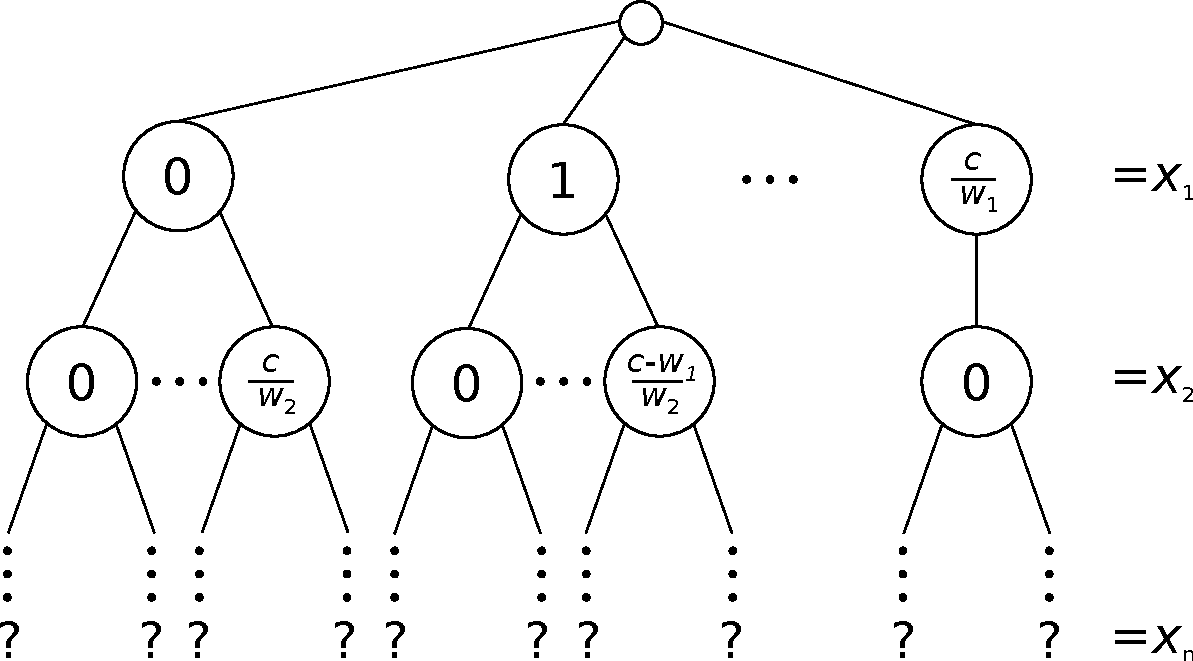
\includegraphics[scale=1]{data/mtu1.pdf}
}
\frame{\frametitle{MTU2 (C++ vs Fortran)}
\includegraphics[scale=1]{data/mtu2.pdf}
}

\subsection{BREQ}
\frame{\frametitle{BREQ}
\includegraphics[scale=1]{data/breq_exp.pdf}
}

\subsection{CSP}

\frame{\frametitle{Time spent solving pricing problems}
\includegraphics[scale=1]{data/pricing_time.pdf}
}

\frame{\frametitle{Time spent solving pricing problems (\% of total time)}
\includegraphics[scale=1]{data/pricing_percentage.pdf}
}

\subsection{Serial Runs vs Parallel Runs}
\frame{\frametitle{Serial Runs vs Parallel Runs}
\includegraphics[scale=1]{data/env_influence.pdf}
}

\mysection{Final Remarks and Future Works}

\subsection{Final Remarks}
\frame{\frametitle{Final remarks}
\begin{itemize}
\setlength\itemsep{1.5em}
\item An algorithm (very similar to one) of 1966 is ``faster'' than the ``state-of-the-art''.
\item Different approaches have advantage over different datasets.
	\begin{itemize}
	\item Artificial datasets and real-world datasets can have different `best algorithms'.
	\end{itemize}
\item The worst-case performance of the \emph{de facto} B\&B algorithms for UKP seems problematic.
\end{itemize}
}

\subsection{Future Works}
\frame{\frametitle{Future Works}
\begin{itemize}
\setlength\itemsep{1.5em}
\item Find real-world UKP/CSP/BPP instances?
\item Combine the UKP5/`Ordered Step-Off' with MTU1? % as EDUK2 did with EDUK and MTU2
\item Re-implement EDUK and EDUK2 in C++? % how would be its performance
\item Implement and test Babayev's algorithm? (see \cite{babayev}) % publicado antes do EDUK e nunca reimplementado para comparação, citado por eduk
\item ... % e muitas outras
\end{itemize}
}

\bibliographystyle{splncs03.bst}

\backupbegin
\setbeamertemplate{footline}{}
\begin{frame}[allowframebreaks]{References}
\small
\bibliography{biblio}
\end{frame}
\backupend
\end{document}

